\documentclass[11pt, oneside]{article} 
\usepackage{geometry}
\geometry{letterpaper} 
\usepackage{graphicx}
	
\usepackage{amssymb}
\usepackage{amsmath}
\usepackage{parskip}
\usepackage{color}
\usepackage{hyperref}

\graphicspath{{/Users/telliott_admin/Tex/png/}}
% \begin{center} 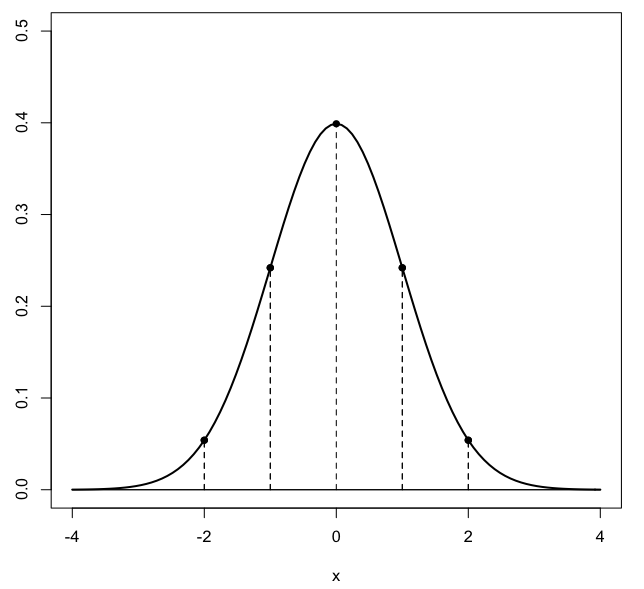
\includegraphics [scale=0.4] {gauss3.png} \end{center}

\title{Introduction}
\date{}

\begin{document}
\maketitle
\Large
\begin{center} 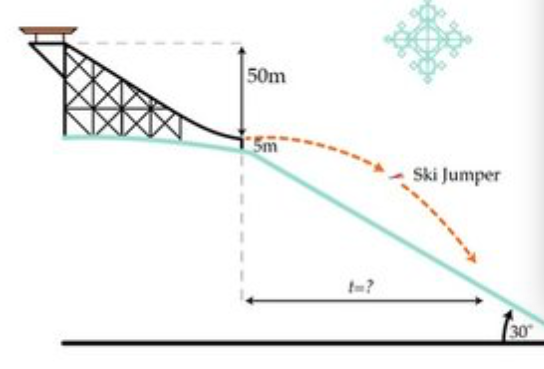
\includegraphics [scale=0.6] {ski_jumper.png} \end{center}
A ski jumper goes down a ramp of 50 meters height which is the same angle as the slope, 30 degrees.  At the very end of the ramp all velocity is converted into horizontal motion by a small lip.  We may not neglect friction:  the coefficient of kinetic friction $\mu = 0.05$.

\subsection*{second part first}

Given some horizontal velocity $v$, the equations of motion (taking $y$ positive downward) are:
\[ x = vt \]
\[ y = \frac{1}{2} gt^2 -5 \]
(We take the origin of coordinates to be 5 m below the release point.)  Solve for the time when
\[ \frac{y}{x} = \tan \theta = \frac{1}{\sqrt{3}} \]
If we can ignore the extra 5 feet, we would have
\[ \tan \theta = \frac{g}{2v} t \]
\[ t = \frac{2v}{g \sqrt{3}} \]
\[ x = v^2 \frac{2}{g \sqrt{3}} = \frac{v^2}{g \cos \theta}  \]
If we cannot neglect it we have
\[ \tan \theta = \frac{g}{2v} t - \frac{5}{vt} \]
\[ \frac{1}{2}gt^2 - v \tan \theta \ t - 5  = 0 \]
Given $v$  we can solve for $t$ and then compute $vt$.

\subsection*{first part}
The force of gravity is $mg$, reduced by the factor of $\cos \theta$.  The force which determines friction is that pointed perpendicular into the slope, $mg \sin \theta$.  Friction opposes gravity along the ramp, giving a net force of
\[ mg \cos \theta - \mu mg \sin \theta \]
The work done is the force times the distance, the length of the ramp, which is $h \sin \theta$.  We have
\[ W = mgh(\cos \theta - \mu \sin \theta) \sin \theta \]
This is equal to the kinetic energy at take-off so
\[ \frac{1}{2} \ mv^2 = mgh(\cos \theta - \mu \sin \theta) \sin \theta \]
\[ v^2 = 2gh(\cos \theta - \mu \sin \theta) \sin \theta \]
so finally
\[ x = \frac{1}{g \cos \theta} \ 2gh(\cos \theta - \mu \sin \theta) \sin \theta \]
\[ = 2h \ (1 - \mu \tan \theta) \sin \theta \]
\[ = 100 \ (1 - \frac{0.05}{\sqrt{3}}) \frac{1}{2} = 50 - \frac{2.5}{\sqrt{3}} \]


\end{document}